\subsection{The computer time}

This section should include the CPU time of the three different methods.



\begin{table}[H]

\begin{tabular}{|c|c|c|c|c|c|}
	\hline
	n & general($ s$)  & special($ s$) & LU(s)  \\ 
\hline  
1e1    &         3.3e-05      &       4.0e-06  &5.5e-04\\ 
1e2    &         3.5e-05      &       1.0e-05  &6.5e-03\\ 
1e3    &         6.1e-05      &       3.9e-05  &3.2e-01\\ 
1e4    &         5.6e-04      &       3.2e-04  &1.4e+02\\ 
1e5    &         9.4e-03      &       3.2e-03  &x\\ 
1e6    &         5.6e-02      &       3.6e-02  &x\\ 
1e7    &         5.9e-01      &       3.6e-01  &x\\ 

	\hline
\end{tabular}
\caption{The total time of the algorithm in the general case, the special case and using LU-decomposition}\label{tab:time}
\end{table}





\hspace{1cm}\linebreak

These numbers are for calculating $n = 10$ to $n = 10^7$ and not printing anything.

Unspecialised: 'CPU time: 2.17188 s'

Specialized: 'CPU time: 2.04688 s'

\subsection{The error}

Too find out how the error developed with the number of mesh points, the step length, we calculated the maximum relative error with different step lengths. The results from these calculations are in Tb. \ref{tab:error_developement} and in Fig. \ref{fig:error_development}. 

\begin{table}[H]\caption{This is a table listing the log of the error and the log of the associated $h$ value. We can see that the smallest error, log(RelativeError) $= -7$, is accomplished when $\log(h) = -4$.}\label{tab:error_developement}
\begin{tabular}{cc}
log(h): & log(RelativeError): \\ \hline
-1.04 & -1.18 \\  \hline
-2.00 & -3.09 \\  \hline
-3.00 & -5.08 \\  \hline
-4.00 & -7.09 \\  \hline
-5.00 & -6.57 \\  \hline
-6.00 & -4.65 \\  \hline
-7.00 & -2.73 \\  \hline

\end{tabular}
\end{table}

\begin{figure}[H]
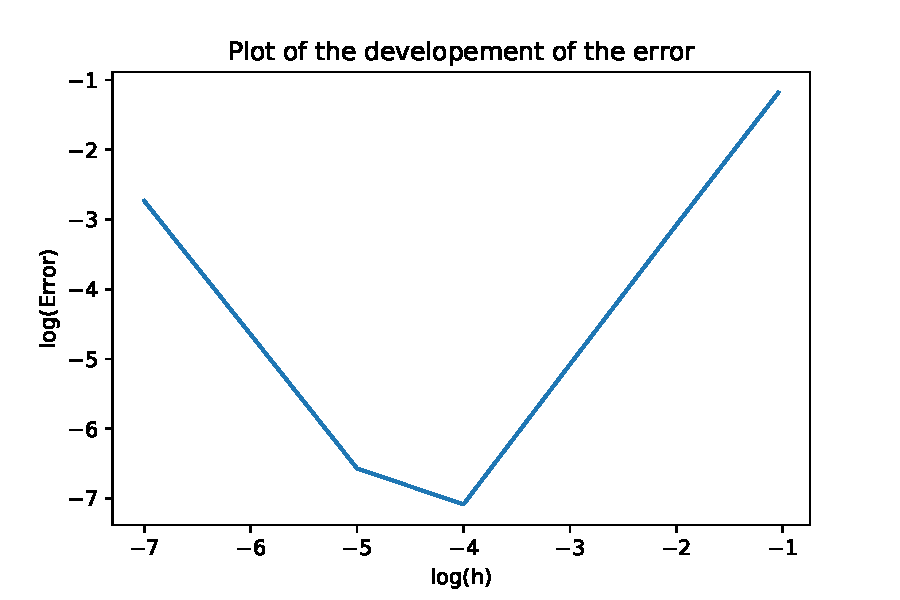
\includegraphics[width=\linewidth]{figures/ErrorDevelopement.pdf}\caption{This is a plot of the log of the error versus the log of the associated $h$ value. We can see that the smallest error, log(RelativeError) $= -7$, is accomplished when $\log(h) = -4$.}\label{fig:error_development}
\end{figure}
